\documentclass[dvipsnames]{beamer}

\usepackage{xcolor}
\usepackage{lmodern}
\usepackage{minted}
\usepackage[utf8]{inputenc}
\usepackage{standalone}
\usepackage{tikz}
\usepackage{caption}
\usepackage{adjustbox}
\usepackage{upquote}
\usepackage{hyperref}
\usepackage{multirow}
\usepackage{booktabs}
\usepackage{array}
\usepackage{xspace}
\usepackage{amssymb}

\usetikzlibrary{mindmap,shadows,arrows,positioning,chains,fit,shapes,decorations.markings}

\usetheme{metropolis}
\usemintedstyle{manni}

\definecolor{gmitblue}{RGB}{20,134,225}
\definecolor{gmitred}{RGB}{220,20,60}
\definecolor{gmitgrey}{RGB}{67,67,67}

\setbeamercolor{structure}{fg=gmitblue}
\setbeamercolor{frametitle}{fg=white, bg=gmitred}
\setbeamercolor{alerted text}{fg=gmitblue}

\renewcommand\footnoterule{}
\newcommand{\citeurl}[1]{\let\thefootnote\relax\footnotetext{\tiny \textcolor{gmitgrey}{\href{http://#1}{#1}}}}

\newcommand{\hr}{\rule{\textwidth}{0.5pt}}

\makeatletter
\expandafter\def\csname PYGdefault@tok@err\endcsname{\def\PYGdefault@bc##1{{\strut ##1}}}
\makeatother

\begin{document}
  \title{Theory of Algorithms}
  \subtitle{}
  \author{ian.mcloughlin@gmit.ie}
  \date{}

  \begin{frame}
    \titlepage
  \end{frame}

  \begin{frame}
    \frametitle{Topics}
    \tableofcontents
  \end{frame}

  %!TEX root = slides.tex

\section{Scheme}

\begin{frame}{John McCarthy}
  \begin{columns}
    \begin{column}{1.5in}
      \includegraphics[width=1.4in]{img/john-mccarthy.png}
    \end{column}
    \begin{column}{0.7\textwidth}
      \begin{itemize}
        \item John McCarthy while at MIT -- late 1950s.
        \vspace{0.25cm}
        \item Created Lisp.
        \vspace{0.25cm}
        \item Lisp generally considered first functional programming language (not really though).
        \vspace{0.25cm}
        \item Lots of dialects exist today, such as Scheme and Common Lisp.
      \end{itemize}
    \end{column}
  \end{columns}
  \citeurl{www-formal.stanford.edu/jmc/}
\end{frame}

\begin{frame}[fragile]{Wasteful for loops}
  \begin{minted}{python}
# How do you parallelise this?
inds = list(range(10))
total = 0
for i in inds:
  total = total + (i * 7)
  \end{minted}
  \begin{minted}{python}
def byseven(i):
  return i * 7

inds = list(range(10))
sevens = map(byseven, inds)
total = sum(sevens)
  \end{minted}
\end{frame}

\begin{frame}{State}
\begin{description}
  \item[Imperative] programming is a programming paradigm where statements are used to change the \emph{state}.
  \item[State] is the name given to the current data/values related to an executing process, including internal stuff like the call stack.
  \item[Processes] begin with an initial state and (possibly) have (a number of) halt states.
  \item[Statements] change the state.
  \item[Functions] in imperative programming languages might return different values for the same input at different times, because of the state.
  \item[Functional] programming languages (try to) not depend on state.
\end{description}
\end{frame}


\begin{frame}{Side effects}
  \begin{description}
    \item[Functions] are said to have side effects if they modify the state (on top of returning a value).
    \item[Static and global] variables are often good examples of side effects in action.
    \item[Functional] programming tries to avoid side effects.
    \item[It's tricky] to avoid them -- such as when we need user input.
  \end{description}
\end{frame}

\begin{frame}[fragile]{Basic operators}
\begin{minted}{scheme}
> (+ 3 4)
7
> (* 3 2)
6
> (- 5 3)
2
> (/ 6 3)
2
\end{minted}
\end{frame}

\begin{frame}[fragile]{More arguments}
\begin{minted}{scheme}
> (+ 3 4 5)
(+ 3 4 5)
> (- 3 4 5)
-6
> (* 2 3 4)
24
> (/ 6 3 3)
2/3
> (/ 6 3 3 3)
2/9
\end{minted}
\end{frame}


\begin{frame}[fragile]{Functions and values}
\begin{minted}{scheme}
; Define a value called foo with value 3.
>(define foo 3)

; Define a function f.  
>(define (f x)
  (+ (* 3 x) 12))

>(define (g x)
  (* 3 (+ x 4)))

>(g 2)
18
\end{minted}
\citeurl{www.artificialworlds.net/presentations/scheme-01-intro/scheme-01-intro.html}
\end{frame}

\begin{frame}[fragile]{Conditionals}
  \begin{minted}{scheme}
> (if (< 1 2) '(y e s) '(n o))
(y e s)

>(define (abs x)
  (if (< x 0)
  (- x)
  x))

\end{minted}
\citeurl{www.artificialworlds.net/presentations/scheme-01-intro/scheme-01-intro.html}
\end{frame}


\begin{frame}[fragile]{Lists}
  \begin{minted}{scheme}
>(list 1 2 3)
(1 2 3)

>(list 'a 'b 'c)
(a b c)

> (length (list 1 2 3))
3
\end{minted}
\citeurl{www.artificialworlds.net/presentations/scheme-01-intro/scheme-01-intro.html}
\end{frame}

\begin{frame}[fragile]{car and cdr}
  \begin{minted}{scheme}
> (car (list 1 2 3))
1
> (cdr (list 1 2 3))
(2 3)
> (define l (list 1 2 3))
> (car l)
1
> (cdr l)
(2 3)
> (car (cdr l))
2
> (cadr l)
2
\end{minted}
\citeurl{www.artificialworlds.net/presentations/scheme-01-intro/scheme-01-intro.html}
\end{frame}

\begin{frame}[fragile]{Recursion}
  \begin{minted}{scheme}
> (define (sum lv)              
    (if (null? lv)
      0
      (+ (car lv) (sum (cdr lv)))))
> (sum (list 1 2 3))                            
6
> (define (derange n)
    (if (= 0 n)
      '()
      (cons n (derange (- n 1)))))
> (derange 12)                                                    
(12 11 10 9 8 7 6 5 4 3 2 1)
\end{minted}
\citeurl{www.artificialworlds.net/presentations/scheme-01-intro/scheme-01-intro.html}
\end{frame}

\begin{frame}[fragile]{Looping recursively}
\begin{minted}{scheme}
> (let loop ((i 5))
(print "i is " i ".\n")
(if (> i 0) (loop (- i 1))))
i is 5.
i is 4.
i is 3.
i is 2.
i is 1.
i is 0.
\end{minted}
\citeurl{gambitscheme.org/wiki/images/a/a7/A\_Tour\_of\_Scheme\_in\_Gambit.pdf}
\end{frame}

\begin{frame}[fragile]{Data and code}
\begin{minted}{scheme}
> (define (swap3-1-2 x)
  (list (cadr x) (car x) (caddr x)))

> (swap3-1-2 (list 1 2 3))
(2 1 3)

> (define four-over-two (list 4 '/ 2))

> four-over-two
(4 / 2)

> (eval (swap3-1-2 four-over-two))
\end{minted}
\citeurl{www.artificialworlds.net/presentations/scheme-01-intro/scheme-01-intro.html}
\end{frame}

\begin{frame}[fragile]{More on functions}
\begin{minted}{scheme}
; Printing stuff to terminal.
> (print "Ay" "-" "yo.\n")
; Proper way to define a function.
> (define foo (lambda (bar) (print "Bar is " bar ".\n")))
; Shorthand.
> (define (foo bar) (print "Bar is " bar ".\n"))

; Local variables.
> (define (foo bar) (let ((thing "Bar"))
    (print thing " is " bar ".\n")))
> (foo "open")
Bar is open.
\end{minted}
\citeurl{gambitscheme.org/wiki/images/a/a7/A\_Tour\_of\_Scheme\_in\_Gambit.pdf}
\end{frame}

\begin{frame}[fragile]{Function example}
  \begin{minted}{scheme}
> (define l 
    (let
      ((d 4) (e 5))
      (lambda (a b c) (list a b c d e))
    )
  )
> (l 1 2 3)
(1 2 3 4 5)
  \end{minted}
  \citeurl{gambitscheme.org/wiki/images/a/a7/A\_Tour\_of\_Scheme\_in\_Gambit.pdf}
\end{frame}

\begin{frame}[fragile]{cons}
\begin{minted}{scheme}
> (cons 1 '())
(1)
> (cons 1 (cons 2 null))
(1 2)
> (cons 1 (cons 2 (cons 3 null)))
(1 2 3)
> (define mylist (cons 1 (cons 2 (cons 3 null))))
> mylist
(1 2 3)
> (car mylist)
1
> (cdr mylist)
(2 3)
\end{minted}
\citeurl{www.artificialworlds.net/presentations/scheme-02-basics/scheme-02-basics.html}
\end{frame}

\begin{frame}[fragile]{More on lists}
\begin{minted}{scheme}
> (list "a" "b" "c")
("a" "b" "c")
> (list a b c)
reference to undefined identifier: a
> (list 'a 'b 'c)
(a b c)

> (equal? 
(list 1 2 3)
(cons 1 (cons 2 (cons 3 '()))))
#t
\end{minted}
\citeurl{www.artificialworlds.net/presentations/scheme-02-basics/scheme-02-basics.html}
\end{frame}

\begin{frame}[fragile]{Quoting}
\begin{minted}{scheme}
> (list a b c)
*** ERROR IN (console)@1.7--Unbound variable: a
> (quote (a b c))
(a b c)
> (quote a b c)
*** ERROR IN (console)@2.1--Ill-formed special form: quote
> '(a b c) 
(a b c)
> (define forty-two '(* 6 9))
> forty-two
(* 6 9)
> (eval forty-two)
54
\end{minted}
\citeurl{www.artificialworlds.net/presentations/scheme-05-quotation/scheme-05-quotation.html}
\end{frame}

\begin{frame}[fragile]{Null list}
\begin{minted}{scheme}
> ()
missing procedure expression
> (list)
()
> '()
()
> null
()
> 'null
null
\end{minted}
\citeurl{www.artificialworlds.net/presentations/scheme-05-quotation/scheme-05-quotation.html}
\end{frame}

\begin{frame}[fragile]{Closures}
\begin{minted}{scheme}
> (define (container value)
(lambda ()
(string-append "This container contains " value ".")))
> (define apple (container "an apple"))
> (define pie (container "a pie"))
> (apple)
"This container contains an apple."
> (apple)
"This container contains an apple."
> (pie)
"This container contains a pie."
\end{minted}
\citeurl{gambitscheme.org/wiki/images/a/a7/A\_Tour\_of\_Scheme\_in\_Gambit.pdf}
\end{frame}
  %!TEX root = slides.tex

\section{Turing machines}


\begin{frame}{Visualisation}
  \begin{adjustbox}{max width={0.9\textwidth},center} 
  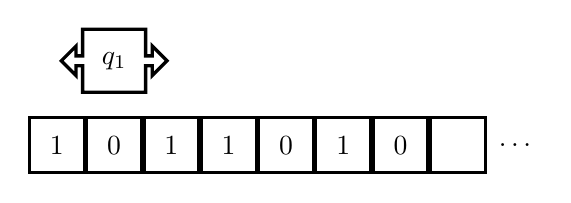
\begin{tikzpicture}
  \tikzstyle{every path}=[very thick]
  
  \edef\sizetape{0.7cm}
  \tikzstyle{tmtape}=[draw,minimum size=\sizetape]
  \tikzstyle{tmhead}=[arrow box,draw,minimum size=.8cm,arrow box arrows={east:.25cm, west:0.25cm}]
  
  \begin{scope}[start chain=1 going right,node distance=-0.15mm]
  \node [on chain=1,tmtape] {1};
  \node [on chain=1,tmtape] (input) {0};
  \node [on chain=1,tmtape] {1};
  \node [on chain=1,tmtape] {1};
  \node [on chain=1,tmtape] {0};
  \node [on chain=1,tmtape] {1};
  \node [on chain=1,tmtape] {0};
  \node [on chain=1,tmtape] {};
  \node [on chain=1,tmtape,draw=none] {$\ldots$};
  \end{scope}

  \node [tmhead,yshift=.7cm] at (input.north) (head) {$q_1$};
  \end{tikzpicture}
  \end{adjustbox}

  \vspace{1.5cm}

  \begin{adjustbox}{max width={0.9\textwidth},center} 
    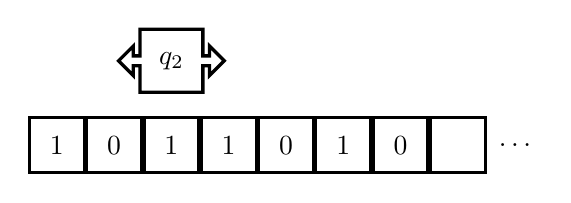
\begin{tikzpicture}
    \tikzstyle{every path}=[very thick]
    
    \edef\sizetape{0.7cm}
    \tikzstyle{tmtape}=[draw,minimum size=\sizetape]
    \tikzstyle{tmhead}=[arrow box,draw,minimum size=.8cm,arrow box arrows={east:.25cm, west:0.25cm}]
    
    \begin{scope}[start chain=1 going right,node distance=-0.15mm]
    \node [on chain=1,tmtape] {1};
    \node [on chain=1,tmtape] {0};
    \node [on chain=1,tmtape] (input) {1};
    \node [on chain=1,tmtape] {1};
    \node [on chain=1,tmtape] {0};
    \node [on chain=1,tmtape] {1};
    \node [on chain=1,tmtape] {0};
    \node [on chain=1,tmtape] {};
    \node [on chain=1,tmtape,draw=none] {$\ldots$};
    \end{scope}
    
    \node [tmhead,yshift=.7cm] at (input.north) (head) {$q_2$};
    \end{tikzpicture}
  \end{adjustbox}
\end{frame}


\begin{frame}{Notation}
\begin{description}
  \item[$Q$] Set of states (finite).
  \item[$G$] Tape alphabet (finite).
  \item[$B$] Blank symbol, element of $G$.
  \item[$S$] Input alphabet, subset of $G \setminus \{ B \} $.
  \item[$\delta$] Transition function.
  \item[$q_0$] Initial state, $\in Q$.
  \item[$q_a$] Accept state, $\in Q$.
  \item[$q_r$] Reject state, $\in Q$.
  \vspace{0.3cm}
  \item[$M$] Turing Machine: $[ Q, G, B, S, \delta , q_0, q_a, q_r ]$.
\end{description}
\end{frame}


\begin{frame}{State Table}
  \begin{table}
    \centering
    \begin{tabular}{cc|ccc}
      \toprule
      State  & Input  & Write & Move & Next \\
      \midrule
      \multirow{3}{*}{0} 
      & B & B &  & Accept \\
      & 0 & 0 & L & 0 \\
      & 1 & 1 & L & 1 \\
      \midrule
      \multirow{3}{*}{1}
      & B & B &  & Fail \\
      & 0 & 0 & L & 1 \\
      & 1 & 1 & L & 0 \\
      \bottomrule
    \end{tabular}
  \end{table}
  
  \[ \delta(q_i, g_n) \rightarrow (q_j, g_m, L/R) \]
\end{frame}


\begin{frame}{Turing's Second Example}
  \begin{block}{A slightly more difficult example}
    We can construct a machine to compute the sequence
    \[ 001011011101111011111 \ldots \]
    The machine is to be capable of five $m$-configurations, viz. $o$, $q$, $p$, $f$, $b$ and of printing $a$, $x$, $0$, $1$.
    The first three symbols on the tape will be $aaO$; the other figures follow on alternate squares.
    On the intermediate squares we never print anything but $x$.
    These letters serve to keep the place for us and are erased when we have finished with them.
    We also arrange that in the sequence of figures on alternate squares there shall be no blanks.
  \end{block}
\end{frame}


\begin{frame}{Turing's Second Example: Table}
  \includegraphics[width=9.5cm]{img/turing-table-2.png}
\end{frame}


\begin{frame}[fragile]{Turing's Second Example: JavaScript 1}
\begin{minted}{javascript}
// The contents of the tape.
var tape = []
s// The current position of the machine on the tape.
var pos = 0
// The current state;
var state = b;
\end{minted}
\end{frame}

\begin{frame}[fragile]{Turing's Second Example: JavaScript 2}
\begin{minted}{javascript}
// Writes a symbol to the current cell on the tape.
function write(sym) {
  tape[pos] = sym;
}

// Returns true iff the current cell contains sym.
function read(sym) {
  return sym == tape[pos] ? true : false;
}
\end{minted}
\end{frame}

\begin{frame}[fragile]{Turing's Second Example: JavaScript 3}
\begin{minted}{javascript}
// Erases the symbol in the current cell of the tape.
function erase() {
  delete tape[pos];
}

// Returns true iff the current cell is blank.
// Returns true iff the current cell is blank.
function blank() {
  return typeof(tape[pos])
    == 'undefined' ? true : false;
}
\end{minted}
\end{frame}

\begin{frame}[fragile]{Turing's Second Example: JavaScript 4}
\begin{minted}{javascript}
function b() {
  write('e');
  pos++;
  write('e');
  pos++;
  write('0');
  pos++;
  pos++;
  write('0');
  pos--;
  pos--;
  state = o;
}
\end{minted}
\end{frame}
  %!TEX root = slides.tex

% 1. Languages
% 2. Deciders
% 3. Big O


\section{Computational complexity}


\begin{frame}{Bubble sort for fixed size input}
  \begin{alertblock}{How many comparisons does bubble sort make for different inputs of the same size?}
    \begin{itemize}
      \item Suppose we have a list with 5 elements.
      \item Best case scenario: list already sorted.
      \item Worst case scenario: list reverse sorted.
    \end{itemize}
    \[ [1,2,3,4,5] \]
    \[ [5,2,1,4,3] \]
    \[ [5,4,3,2,1] \]
  \end{alertblock}
\end{frame}


\begin{frame}{Bubble sort different sized inputs}
  \begin{alertblock}{How many comparisons does bubble sort make for inputs of increasing length?}
    \begin{itemize}
      \item Suppose we have a list with $n$ elements.
      \item Compare the worst case scenario for each value of $n$.
    \end{itemize}
    \[ [3,2,1] \]
    \[ [4,3,2,1] \]
    \[ [5,4,3,2,1] \]
    \[ [6,5,4,3,2,1] \]
  \end{alertblock}
\end{frame}


\begin{frame}{Average vs. worst case}
  \begin{table}
    \begin{tabular}{p{2cm}rr}
      Input & Algorithm A & \hspace{1cm} Algorithm B \\
      \hline
      (1,2,3) &  1ms &  1ms \\
      (1,3,2) &  1ms &  5ms \\
      (2,1,3) &  2ms &  4ms \\
      (2,3,1) &  2ms &  5ms \\
      (3,1,2) &  2ms &  5ms \\
      (3,2,1) & 10ms &  4ms \\
      \hline
      Average &  3ms &  4ms \\
      Worst   & 10ms &  5ms
    \end{tabular}
  \end{table}
  \begin{center}
    Would you choose Algorithm A or Algorithm B?
  \end{center}
\end{frame}


\begin{frame}{Terminology of complexity}
  \begin{alertblock}{How does the number of operations change as $n$ increases?}
    \begin{description}
      \item[Linear] Multiply $n$ by a constant, add a constant. (Special category of polynomial time.)
      \item[Polynomial] Multiply $n$ by itself a fixed number of times, multiply by a constant. (Can add such terms together.)
      \item[Exponential] Raise a constant to the power of $n$. (Rate of change is still exponential.)
      \item[Logarithmic] Opposite of exponential.
    \end{description}
  \end{alertblock}
\end{frame}


\begin{frame}[fragile]{Terminology of complexity (graph)}
\begin{center}
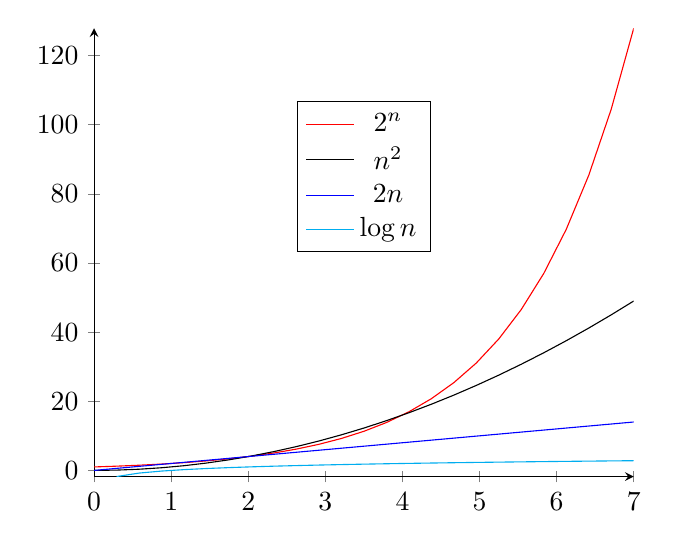
\begin{tikzpicture}
  \begin{axis}[xmin=0, domain=0:7, axis x line=bottom, axis y line=left, legend style={at={(0.5,0.5)},anchor=south}]
    \addplot[red]   {pow(2,x)};
    \addplot[black] {pow(x,2)};
    \addplot[blue]  {2*x};
    \addplot[cyan]  {ln(x)/ln(2))};
    \legend{$2^n$,$n^2$,$2n$,$\log n$};
  \end{axis}
\end{tikzpicture}
\end{center}
\end{frame}


\begin{frame}{Linear}
  \[ f(n) = a_0 + a_1 n \]
  \begin{alertblock}{How many pairs of shoes does a centipede need?}
    \begin{itemize}
      \item Let's say a centipede has 100 feet.
      \item Then every centipede needs 100 shoes.
      \item That's 50 pairs of shoes.
      \item So 2 centipedes need 100 pairs, 3 need 150 pairs, etc.
      \item So $n$ centipedes need $50n$ pairs of shoes.
      \item Linearity is familiar, and most people's default assumption.
      \item You take the input, multiply by a constant, and add another constant.
    \end{itemize}
  \end{alertblock}
\end{frame}


\begin{frame}{Polynomial}
  \[ f(n) = a_0 + a_1 n + a_2 n^2 + a_3 n^3 + \ldots \]
  \begin{alertblock}{What is the volume of a cube of side $n$?}
    \begin{itemize}
      \item Suppose we have a cube with sides of length 1 metre.
      \item The volume of the cube is $1 \times 1 \times 1 = 1$ metres cubed.
      \item Suppose the cube has sides of length 2 metres instead.
      \item The volume of the cube is $2 \times 2 \times 2 = 8$ metres cubed.
      \item In general, for sides of length $n$, the volume is $n^3$.
    \end{itemize}
  \end{alertblock}
\end{frame}


\begin{frame}{Exponential}
  \[ f(n) = a^n \]
  \begin{alertblock}{How many numbers can we represent with $n$ bits?}
    \begin{itemize}
      \item Consider the case of four bits -- imagine four placeholders \textbf{\fbox{?}}\textbf{\fbox{?}}\textbf{\fbox{?}}\textbf{\fbox{?}}
      \item Each placeholder can contain either 0 or 1.
      \item There are $2 \times 2 \times 2 \times 2 = 2^4 = 16$ different numbers.
      \item Add another bit, how many numbers is it now?
      \item It's $2 \times 2 \times 2 \times 2 \times 2 = 2^5 = 32$.
      \item Generally $n$ bits can represent $2^n$ numbers.
    \end{itemize}
  \end{alertblock}
\end{frame}


\begin{frame}{Logarithmic}
  \[ f(n) = \log_a n \]
  \begin{alertblock}{How many bits do we need to represent $n$ numbers?}
    \begin{itemize}
      \item If we have $n$ bits we can represent $2^n$ numbers.
      \item If we want to represent $n$ numbers, how many bits to we need (at a minimum)?
      \item The inverse operation to exponentiation is logarithm.
      \item Remember, $a^n = b$ means $\log_a b = n$.
    \end{itemize}
  \end{alertblock}
\end{frame}

\begin{frame}{Big-O (Sipser)}
  \begin{definition}
    Let $f$ and $g$ be functions $f,g: \mathbb{N} \rightarrow \mathbb{R}^+$.
    We say that $f(n) = O(g(n))$, or $f$ is \emph{big-O} of $g$, if positive integers $c$ and $n_0$ exist such that, for every integer $n$ greater than or equal to $n_0$, $f(n) \le cg(n)$.
  \end{definition}
  \begin{alertblock}{Example}
    Let $f$ be the function $f(n) = 5n^3 + 2n^2 + 22n + 6$.
    We'll prove that $f$ is big-O of $n^3$ ($f = O(n^3)$).
    Let $c$ be $6$ and $n_0$ be $10$.
    Is the following true, for all $n$ greater than or equal to 10, $5n^3 + 2n^2 + 22n + 6 \le 6n^3$?
    Note that as $n$ increases ($n=10,n=11,n=12,\ldots$), $f(n)$ also increases.
    Also note that $f(10) = 5426$ and $6g(10) = 6000$.
  \end{alertblock}
  \citeurl{math.mit.edu/~sipser/book.html}
\end{frame}


\begin{frame}[fragile]{Big-O example graph}
\begin{center}
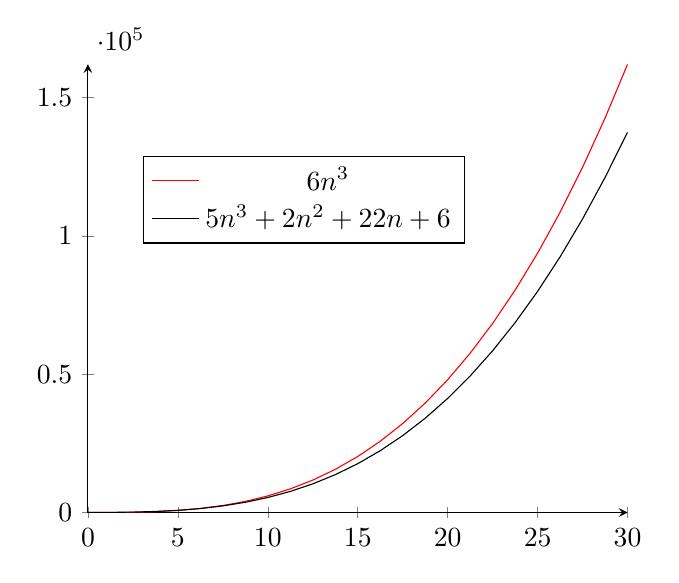
\begin{tikzpicture}
  \begin{axis}[xmin=0, domain=0:30, axis x line=bottom, axis y line=left, legend style={at={(0.4,0.6)},anchor=south}]
    \addplot[red]   {6*pow(x,3)};
    \addplot[black] {5*pow(x,3) + 2*pow(x,2) + 22*x + 6};
    \legend{$6n^3$,$5n^3 + 2n^2 + 22n + 6$};
  \end{axis}
\end{tikzpicture}
\end{center}
\end{frame}

\begin{frame}[fragile]{Smaller values of $n$}
\begin{center}
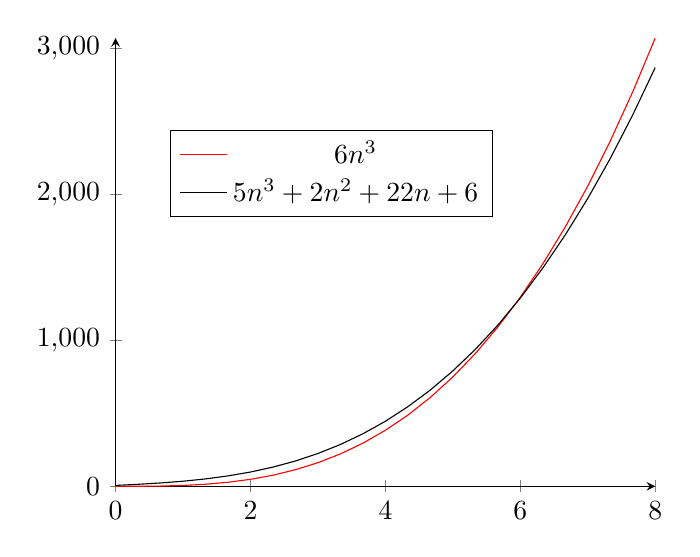
\begin{tikzpicture}
  \begin{axis}[xmin=0, domain=0:8, axis x line=bottom, axis y line=left, legend style={at={(0.4,0.6)},anchor=south}]
    \addplot[red]   {6*pow(x,3)};
    \addplot[black] {5*pow(x,3) + 2*pow(x,2) + 22*x + 6};
    \legend{$6n^3$,$5n^3 + 2n^2 + 22n + 6$};
  \end{axis}
\end{tikzpicture}
\end{center}
\end{frame}

\begin{frame}[fragile]{Bubble sort is $O(n^2)$}
\begin{center}
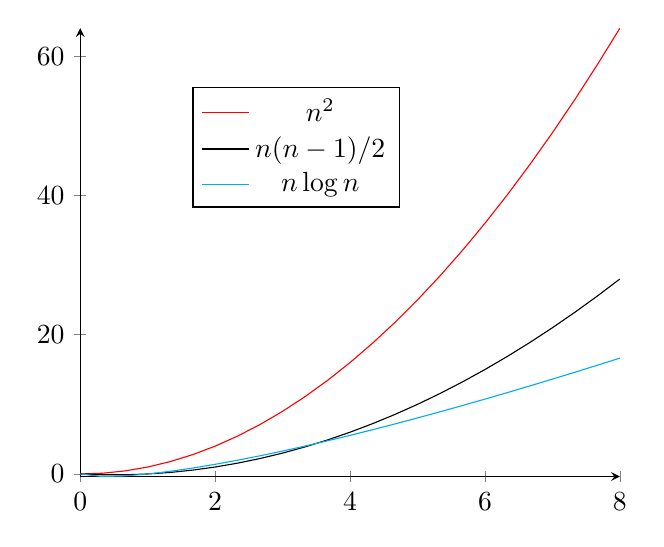
\begin{tikzpicture}
  \begin{axis}[xmin=0, domain=0:8, axis x line=bottom, axis y line=left, legend style={at={(0.4,0.6)},anchor=south}]
    \addplot[red]   {x^2};
    \addplot[black] {x*(x-1)/2};
    \addplot[cyan]   {x*ln(x)};
    \legend{$n^2$,$n(n-1)/2$,$n \log n$};
  \end{axis}
\end{tikzpicture}
\end{center}
\end{frame}


\begin{frame}{Polynomial time}
  \begin{definition}
    An algorithm is said to be solvable in \emph{polynomial time} if the number of steps required to complete the algorithm for a given input is $O(n^k)$ for some nonnegative integer $k$, where $n$ is the complexity of the input.
  \end{definition}
  \vspace{0.5cm}
  \metroset{block=fill}
  \begin{block}{$P$ complexity class}
    The $P$ complexity class is the set of problems for which there exists, for each such problem, at least one algorithm to solve that problem in polynomial time.
  \end{block}

  \citeurl{mathworld.wolfram.com/P-Problem.html}
\end{frame}


\begin{frame}{Polynomial time on a Turing machine}
  \begin{description}
    \item[Sorting] algorithms are usually compared in terms of comparisons.
    \item[Other algorithms] might be compared in terms of something else, like iterations.
    \item[With Turing machines] we can use the number of times we look up the state table.
    \item[The size] of the input can be the length of the input on the tape initially.
  \end{description}
\end{frame}


\begin{frame}{Recap on Languages}
  \begin{description}
    \item[Alphabet] Finite set of symbols, denoted $\Sigma$.
    \item[String] Sequence of symbols, $w$ from $\Sigma$.
    \item[Language] Set of strings, denoted $L$.
    \item[Length] Of a string, denoted $|w|$  .
    \item[Empty string] Unique string of length 0, denoted $\epsilon$.
  \end{description}
\end{frame}


\begin{frame}{Kleene star}
  \begin{description}
    \item[Word concatenation:] $w_1 w_2$ is the concatenation of strings $w_1$ and $w_2$.
    \item[String concatenation:] $L_1 L_2$ is the language resulting from the concatenation of all strings in $L_1$ and all words in $L_2$, in that order.
    \item[Powers:] $L^0 = \{ \lambda \}$, $L^1 = L$ and $L^{n+1} = L^n L$ for all $n > 1$.
  \end{description}
  \vspace{0.5cm}
  \begin{block}{Kleene Star}
     \[ L^* =  \bigcup_{i=0}^{\infty} L^i \]
  \end{block}
  Note that treating the alphabet $\Sigma$ as a language in itself, we get that $\Sigma^*$ is the set of all words over $\Sigma$.
\end{frame}


\begin{frame}{Example}
  \begin{description}
    \item[$\Sigma$] $\{ 0, 1 \}$
    \item[$L$] $\{ 00, 01, 10, 11 \}$
    \item[$w_1$] $01$
    \item[$w_3$] $11$
    \item[$w_1 w_3$] $0111$
    \item[$\Sigma^*$] $\{ \lambda, 0, 1, 00, 01, 10, 11, 001, 010, \ldots \}$
    \item[$L^*$] $\{ \lambda, 00, 01, 10, 11, 0000, 0001, \ldots \}$
    \item[$L^+$] $\{ 00, 01, 10, 11, 0000, 0001, \ldots \}$
  \end{description}
\end{frame}

\begin{frame}{Think about $\{0,1\}^*$}
  Consider the set:
  \[ \Sigma^* \quad \textrm{where} \quad \Sigma = \{0,1\} \]
  \vspace{1mm}
  \begin{description}
    \item[$\Sigma^*$]  is the set of all strings (of all lengths) of 0's and 1's.
    \item[Documents] on a computer are elements of $\Sigma^*$.
    \item[Programs] on a computer are elements of $\Sigma^*$.
    \item[The entire contents] of your hard drive is one big string of 0's and 1's, and so is in $\Sigma^*$.
  \end{description}
\end{frame}

\begin{frame}[fragile]{Example of a text file}
Create a text file on your computer with this single line of text:
  \begin{minted}{text}
Hello I'm a text file!
  \end{minted}
  Then open it in a hex editor and see this:
  \begin{minted}{text}
48656C6C6F2049276D206120746578742066696C6521
  \end{minted}
  The hex editor is just displaying the binary as hex:
  \begin{minted}{text}
01001000011001010110110001101100011011110010
00000100100100100111011011010010000001100001
00100000011101000110010101111000011101000010
00000110011001101001011011000110010100100001
  \end{minted}
\end{frame}


\begin{frame}{Decision problems}
  \begin{description}
    \item[Decision problems] are problems where the answer is 0 or 1.
    \[ f:\{0,1\}^n \rightarrow \{0,1\} \]
    \item[Turing machines] model decision problems by deciding languages.
    \vspace{0.1cm}
    \item[Deciders] are Turing machines that decide languages -- they end in an accept or fail state no matter what the input, as opposed to never finishing.
    \vspace{0.1cm}
    \item[Accept] is 1, fail is 0.
  \end{description}
\end{frame}

\begin{frame}{Deciding Word documents}
  \begin{alertblock}{Can a Turing machine decide valid Word documents?}
    Word documents are just strings of 0's and 1's, elements of $\{0,1\}^*$.
    Not all strings of 0's and 1's are valid Word documents.
    
    If you try to open any old string of 0's and 1's in Word, it will likely tell you your file is corrupt.
    
    Can we construct a Turing machine that accepts all valid Word documents, and fails otherwise?
    
    Word seems to be able to decide what a valid Word document is, but it's always dealing with finite inputs.
    The specification might allow for infinite Word documents.
  \end{alertblock}
\end{frame}

\begin{frame}{PRIMES}
  \begin{definition}
    $$ PRIMES = \{ 2, 3, 5, 7, 11, 13, ... \} $$
  \end{definition}
  \begin{description}
    \item[PRIMES] is the set of all primes numbers.
    \item[Can] a Turing Machine be designed to decide PRIMES? (Yes)
    \item[Some] people say PRIMES is the decision problem for the set of primes.
    \item[Can] it do it in polynomial time? (Yes)
    \item[Is] PRIMES in P? (Yes, 2002)
  \end{description}
  \citeurl{www.cse.iitk.ac.in/users/manindra/algebra/primality\_v6.pdf}
\end{frame}

\begin{frame}{Modern cryptography}
  \begin{alertblock}{Modern asymmetric key crytography is based on prime numbers}
    It depends on two facts:
    \begin{itemize}
      \item It's easy to verify primes (P).
      \item It's hard to decompose a composite number into primes (Not known to be P).
    \end{itemize}
  \end{alertblock}
  \begin{alertblock}{Generating versus verifying}
    Note that it's not neccessarily easy to generate prime numbers.
    We know that verifying a number is prime can be done in polynomial time.
    That doesn't mean that we can generate prime numbers in polyonmial time.
    You have to start with the prime, and then ask the question.
  \end{alertblock}

\end{frame}

\begin{frame}[fragile]{Brute force prime checking}
  \begin{alertblock}{Is n a prime?}
    \begin{minted}{c}
function is_prime(n) {
  for (var i = 2; i < n; i++) {
    if (n % i == 0)
      return false;
  }
  return true;
}
    \end{minted}
  \end{alertblock}
\end{frame}

\begin{frame}[fragile]{More efficient prime checking}
  \begin{itemize}
    \item Suppose $a \times b = n$.
    \item Then $a < b$, $a > b$ or $a = b$.
    \item No matter what, $a \le \sqrt{n}$ and/or $b \le \sqrt{n}$.
    \item So only loop to $\sqrt{n}$.
    \item This still isn't that efficient.
  \end{itemize}
\end{frame}

\begin{frame}[fragile]{Slightly more efficient}
  \begin{alertblock}{Is n a prime?}
    \begin{minted}{c}
function is_prime(n) {
  for (var i = 2; i < Math.sqrt(n); i++) {
    if (n % i == 0)
      return false;
  }
  return true;
}
    \end{minted}
  \end{alertblock}
\end{frame}

%\begin{frame}[fragile]{AKS prime checking (2002)}
%  \begin{enumerate}
%    \item If $n = a^b$ where $a,b \in \mathbb{N}^+$, output composite.
%    \item Find the smallest $r$ such that $ord_r(n) > (log_2 n)^2$.
%    \item No matter what, $a \le \sqrt{n}$ and/or $b \le \sqrt{n}$.
%    \item So only loop to $\sqrt{n}$.
%    \item This still isn't that efficient.
%  \end{enumerate}
%  \citeurl{wikipedia.org/wiki/AKS\_primality\_test}
%\end{frame}
  %!TEX root = slides.tex

\section{NP completeness}


\begin{frame}{Non-deterministic polynomial time}
  \begin{definition}
  A problem is in the $NP$ complexity class if it is solvable by a non-deterministic Turing Machine in polynomial time. A non-deterministic Turing Machine is one which may not have a unique action to take for some or all states and inputs.
  \end{definition}
  
  \vspace{0.5cm}
  \metroset{block=fill}
  \begin{block}{$P$ is a subset of $NP$}
  The $P$ complexity class is a subset of $P$ because all polynomial time solvabled problems can be modelled using Nondeterministic Turing Machinses.
  \end{block}

  \citeurl{mathworld.wolfram.com/P-Problem.html}
\end{frame}


\begin{frame}{$NP$-complete problems}
  \begin{definition}
    An problem is $NP$-hard if each problem in $NP$ can be reduced to it in polynomial time.
  \end{definition}
  
  \vspace{0.5cm}
  {\metroset{block=fill}
  \begin{block}{$NP$-hard problems are hard}
  $NP$-hard problems are at least as hard to solve as the hardest $NP$ problems.
  Note that $NP$-hard problems don't have to be $NP$.
  \end{block}}
  
  \vspace{0.5cm}
  \begin{definition}
    An problem is $NP$-complete if it's in $NP$ and in $NP$-hard.
  \end{definition}
\end{frame}


\begin{frame}{Subset sum problem}
   
   {\metroset{block=fill}
  \begin{block}{Problem}
    Given a set of integers $S$, is there a non-empty subset whose elements sum to zero?
  \end{block}}

  \vspace{0.5cm}
  
  \begin{block}{Example}
    Does $\{ 1, 3, 7, -5, -13, 2, 9, -8 \}$ have such a subset?
  \end{block}
  
  \vspace{0.5cm}

  \begin{block}{Note}
     If somebody suggests a soltuion, it is very quick to check it.
    Being able to quickly verify a solution is a characteristic of $NP$ problems.
  \end{block}
\end{frame}


\begin{frame}{Propositional logic}
  \begin{description}
    \item[Literals] are Boolean variables (can be True or False), and their negations. They are represented by lower case letters like $a$ and $x_i$.
    \vspace{0.3cm}
    \item[Clause] are expressions based on literals, that evaluate as True or False based on the literals. We use not, and and or on the literals. We'll sometimes call them expressions.
    \vspace{0.3cm}
    \item[Not] is depicted by $\neg$. So ``not $a$'' is denoted by $\neg a$.
    \vspace{0.3cm}
    \item[Or] is depicted by $\vee$. So ``$a$ or $b$'' is denoted by $a \vee b$.
    \vspace{0.3cm}
    \item[And] is depicted by $\wedge$. So ``$a$ and $b$'' is denoted by $a \wedge b$.
  \end{description}
\end{frame}


\begin{frame}{Normal forms}
  \begin{description}
    \item[CNF] A clause is in Conjunctive Normal Form if it is a ``conjunction of disjunctions'': $(a \vee b) \wedge (\neg a \vee c) \wedge d$.
    \vspace{0.5cm}
    \item[DNF] A cluse is in Disjunctive Normal Form if it is a ``disjunction of conjunctions'': $(a \wedge b) \vee (\neg a \wedge c) \vee d$.
  \end{description}
  \vspace{0.5cm}
  {\metroset{block=fill}\begin{block}{Converting to CNF and DNF}
    Every Boolean expression can be converted to CNF, and every Boolean expression can also be converted to DNF.
  \end{block}}
\end{frame}


\begin{frame}{Four laws}
  The following four laws can be used to convert expressions to CNF and DNF.
  The first two are known as De Morgan's laws, and the latter two are called the distributivity laws.
  \vspace{0.5cm}
  {\metroset{block=fill}\begin{block}{Conversion laws}
    \[ \neg ( a \vee b) = \neg a \wedge \neg b \]
    \[ \neg ( a \wedge b) = \neg a \vee \neg b \]
    \[ c \wedge ( a \vee b) = (c \wedge a) \vee (c \wedge b) \]
    \[ c \vee ( a \wedge b) = (c \vee a) \wedge (c \vee b) \]
  \end{block}}
\end{frame}


\begin{frame}{Boolean Satisfiability Problem (SAT)}
  {\metroset{block=fill}
    \begin{block}{The problem}
    We're often interested in knowing if there is any setting of the variables in a Boolean expression that makes the expression true.
    Another way of asking the question is: is the expression satisfiable?
    The real question is, is there a polynomial time algorithm that takes as input \emph{any} Boolean expression and outputs true if there is any setting, and false otherwise.
  \end{block}}
  \vspace{0.5cm}
  The problem is the prototypical NP-complete problem.
  Note that it's quick to check the correctness of a solution for a given expression. 
\end{frame}


\begin{frame}{CNF SAT}
  
  {\metroset{block=fill}
    \begin{block}{Only using CNF}
    All Boolean expressions can be converted in CNF.
    However, it's not always possible to do that in polynomial time.
    We can though, in polynomial time, create new expressions using some extra(neous) variables that are satisfiable if and only if the original expression is.
  \end{block}}
  \vspace{0.5cm} 
\end{frame}


\begin{frame}{$k$-SAT}
  
  {\metroset{block=fill}
    \begin{block}{$k$-SAT}
     $k$-SAT is like SAT except that all expressions must be in CNF and each clause must be a disjunction of $k$ literals.
  \end{block}}
  \vspace{0.25cm}
  \begin{description}
  \item[2-SAT] $(a \vee b) \wedge (\neg c \vee d) \wedge \ldots$
  \vspace{0.25cm}
  \item[3-SAT] $(a \vee b \vee c) \wedge (\neg c \vee d \vee \neg a) \wedge \ldots$
  \end{description}
    \vspace{0.25cm}
   \begin{description}
     \item[2-SAT] is not NP-complete. There are polynomial time algorithms that solve it.
     \vspace{0.25cm}
     \item[3-SAT] is NP complete.
   \end{description}
\end{frame}


\begin{frame}{3-SAT is NP-Complete}

  {\metroset{block=fill}
    \begin{block}{Reduction}
    3-SAT is a special case of SAT, so 3-SAT must be in NP.
    We can reduce SAT to 3-SAT in polynomial time.
    First take the expression and convert it to a CNF expression (in polynomial time).
    Then we just need to convert each clause into a CNF expression with 3 literals per clause.
    
    Suppose we have a clause with 1 literal: $a$.
    Convert this to $(a \vee u_1 \vee u_2) \wedge (a \vee u_1 \vee \neg u_2) \wedge (a \vee \neg u_1 \vee u_2) \wedge (a \vee \neg u_1 \vee \neg u_2)$.
    Suppose we have a clause with 2 literals: $a \vee b$.
    Convert this to $(a \vee b \vee u_1) \wedge (a \vee b \vee \neg u_1))$.
    
    Now suppose we have a clause with $n$ literals: $a \vee b \vee c \vee \ldots$.
    Convert this to $(a \vee b \vee u_1) \wedge (c \vee \neg u_1 \vee u_2)) \wedge \ldots \wedge (i \vee \neg u_{n-4} \vee u_{n-3}) \wedge (j \vee k \vee \neg u_{n-3})$.
  \end{block}}

\end{frame}
\end{document}
 